\documentclass[tikz,border=8pt]{standalone}
% Shared look for every TikZ diagram. Load with \input{../../tools/tikz-style.tex}
\usepackage[T1]{fontenc}
\usepackage{lmodern}
\renewcommand{\sfdefault}{lmr}  % diagrams use the same serif as the text
\usetikzlibrary{arrows.meta, positioning, shapes.geometric, calc, fit, backgrounds}
\definecolor{cblue}{HTML}{4C78A8}
\definecolor{corange}{HTML}{F58518}
\definecolor{cgreen}{HTML}{54A24B}
\definecolor{cred}{HTML}{E45756}
\definecolor{cpurple}{HTML}{B279A2}
\definecolor{cgrey}{HTML}{6B6B6B}
\tikzset{
  every picture/.style={font=\sffamily, line width=1.2pt},
  box/.style={draw=#1, fill=#1!12, rounded corners=4pt, align=center, inner sep=7pt, minimum height=1.1cm},
  box/.default=cgrey,
  arrow/.style={-{Stealth[length=3mm]}, draw=cgrey, line width=1.4pt},
  title/.style={font=\sffamily\bfseries\Large},
  note/.style={font=\sffamily\small, text=cgrey, align=center},
}
\AtBeginDocument{\hyphenpenalty=10000 \exhyphenpenalty=10000}

% The set-valued information state and the belief update in the same two steps. A move: union of reachable states
% becomes a sum over previous states (law of total probability). A reading: intersection with the states that fit
% becomes multiply by p(z | x) and rescale (Bayes' theorem).
\begin{document}
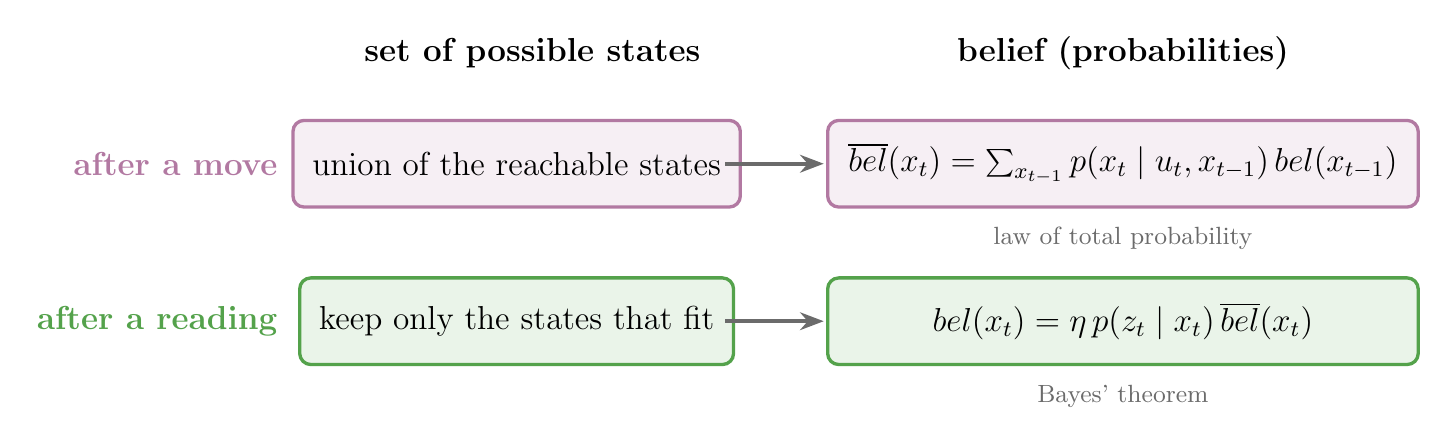
\begin{tikzpicture}[x=1cm, y=1cm, every node/.append style={font=\large}]
  \node[font=\large\bfseries] at (2.5,3) {set of possible states};
  \node[font=\large\bfseries] at (10,3) {belief (probabilities)};
  \node[cpurple, anchor=east, font=\large\bfseries] at (-0.6,1.6) {after a move};
  \node[cgreen, anchor=east, font=\large\bfseries] at (-0.6,-0.4) {after a reading};
  \node[box=cpurple, minimum width=4.9cm] at (2.3,1.6) {union of the reachable states};
  \node[box=cpurple, minimum width=7.5cm] at (10,1.6) {$\overline{\text{bel}}(x_t) = \sum_{x_{t-1}} p(x_t \mid u_t, x_{t-1})\,\text{bel}(x_{t-1})$};
  \node[box=cgreen, minimum width=4.9cm] at (2.3,-0.4) {keep only the states that fit};
  \node[box=cgreen, minimum width=7.5cm] at (10,-0.4) {$\text{bel}(x_t) = \eta\, p(z_t \mid x_t)\,\overline{\text{bel}}(x_t)$};
  \draw[arrow] (4.95,1.6) -- (6.2,1.6);
  \draw[arrow] (4.95,-0.4) -- (6.2,-0.4);
  \node[note] at (10,0.65) {law of total probability};
  \node[note] at (10,-1.35) {Bayes' theorem};
\end{tikzpicture}
\end{document}
